\newchapt{Slice Enhancement}{chapt3}{Slice Enhancement}

%%%%%%%%%%%%%%%%%%%%%%%%%%%%%%%%
%%%%%%   Slice Enhancement  %%%%
%%%%%%%%%%%%%%%%%%%%%%%%%%%%%%%%
\section{Hole Filling}
\label{sec:mdr}

The slices we extract above often have holes (i.e., missing data) due to
occlusion or other visibility issues.
Fortunately, most urban buildings have symmetry that we can exploit to
fill these holes.
Symmetry computation on 3D data is an active research topic, such as those in
\cite{Sym_PSGRF,Sym_ZPA,Sym_TW,Sym_MGP}, which has potentially numerous applications.
However, symmetry computation 3D data directly is expensive. 
Here, we only conduct this computation on the 2D image slices.
Since the 3D data has been already rectified \cite{RDP_LSYGS} and projected onto 2D slices, hence only 2D translation
is needed to be considered for symmetry computation.
Let $P(x,y)$ be a point on the original image $I$ and $P'(x',y')$ be the reflected
point of $P$ with respect to a symmetry line $L$.
The symmetry computation equation for $L$ is as follows:
\begin{equation}
L = \underset{x,y}{\operatorname{arg\,min}}\sum{d_{x,y}(P', I)}
\end{equation}
where the $d_{x,y}(P',I)$ is the distance between the self-reflected point
$P'$ and its nearest data point in image $I$.
The reflected point $P'$ of the original point $P$ is computed with
respect to a line along either the $x-$ or $y-$ axis.
Therefore, the symmetry line $L$ is obtained as the line with minimum
summation error over the reflected data points.
\Figa{sym} and \Figb{sym} depict the original input with holes, and
the output after hole filling using symmetry computation, respectively.

\begin{figure}[htbp]
\begin{center}
\begin{tabular}{c}
\fbox{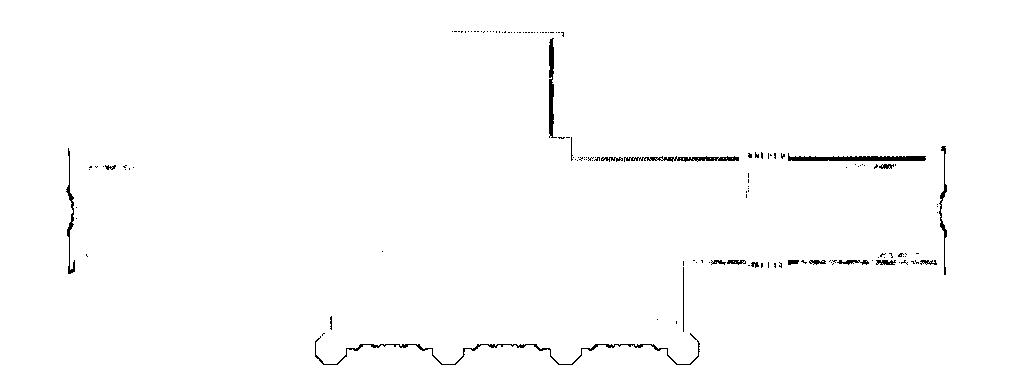
\includegraphics[width=0.6\textwidth]{image_slice_0705_0711.png}} \\
(a) \\
\fbox{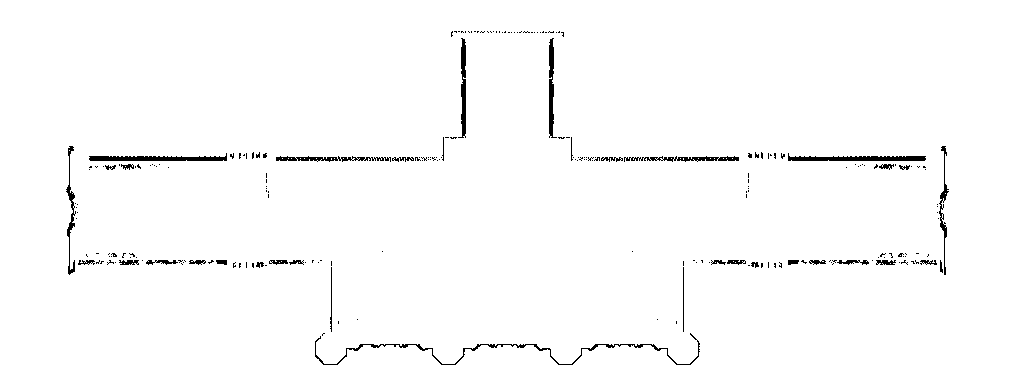
\includegraphics[width=0.6\textwidth]{image_slice_0705_0711_recoverd.png}} \\
(b)
\end{tabular}
\end{center}
\caption{ Symmetry-based hole filling. (a) Original 2D slice image and
(b) output image after hole filling.}
\label{fig:sym}
\end{figure}

